\documentclass{beamer}
\usetheme[hideothersubsections]{HRTheme}
\usepackage{beamerthemeHRTheme}
\usepackage{graphicx}
\usepackage[space]{grffile}
\usepackage{listings}
\usepackage{animate}
\lstset{language=SQL,
basicstyle=\ttfamily\footnotesize,
mathescape=true,
keywordstyle=\color{blue},
breaklines=true,
showspaces=false,
showstringspaces=false}
\usepackage[utf8]{inputenc}
\usepackage{color}
\newcommand{\red}[1]{
\textcolor{red}{#1}
}
\newcommand{\ts}{\textbackslash}

\title{Indexing and Query optimization}

\author{ }

\institute{Hogeschool Rotterdam \\ 
Rotterdam, Netherlands}

\date{}

\begin{document}
\maketitle

\SlideSection{Introduction}
\SlideSubSection{Lecture topics}
\begin{slide}{
\item Query optimization.
\item Examples of slow query operations.
\item Hashing.
\item Trees.
}\end{slide}

\SlideSection{Query optimization}
\SlideSubSection{Reasons}
\begin{slide}{
\item Query needs to be fast.
\item Sometimes they are not.
\item You do not want to see your nephew born before retrieving the book you are looking for from Amazon.

\begin{figure}
\centering
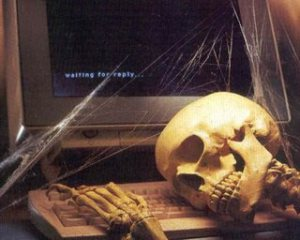
\includegraphics[scale=0.35]{img/skeleton_computer}
\end{figure}
}\end{slide}

\SlideSubSection{Causes}
\begin{slide}{
\item Too much data (Big data analysis).
	\begin{itemize}
	\item Data clustering.
	\item Better hardware. (arrays of disks, caching, ...)
	\end{itemize}
\item Too complex queries (DBMS optimization)
	\begin{itemize}
	\item Refactor query. (Access planner)
	\item Refactor data. (Indexing)
	\end{itemize}
}\end{slide}

\SlideSubSection{Indexes}
\begin{slide}{
\item Query refactoring not always possible.
\item Build additional data to speed up the data retrieval.
}\end{slide}

\SlideSubSection{Indexes}
\begin{slide}{
\item Take your text book and look for the paragraph titled ``Key constraints'' without using the index. How many pages have you looked?
\pause
\item \textbf{Answer:} 29 (from page 3 to 32).
\pause
\item Do the same using the index. How many pages have you looked?
\pause
\textbf{Answer:} 2 (1 in the index, 1 in the text).
}\end{slide}

\SlideSection{Problematic queries}
\begin{frame}[fragile]{Where}
\begin{lstlisting}
SELECT name
FROM ships
WHERE firepower = 1500
\end{lstlisting}
\tiny
\begin{tabular}{|c|c|c|c|c|}
\hline
\multicolumn{5}{|c|}{\textbf{ships}} \\
\hline
name & type & firepower & speed & position \\
\hline
Red 1 & X-Wing & 10 & 300 & (1,3,1) \\
\hline
Red 2 & X-Wing & 10 & 300 & (1,2,1) \\
\hline
Red 3 & X-Wing & 10 & 300 & (0,2.5,1) \\
\hline
Red 4 & X-Wing & 10 & 300 & (2,2.5,1) \\
\hline
Red 5 & X-Wing & 10 & 300 & (2,2.5,0) \\
\hline
Red 6 & X-Wing & 10 & 300 & (1,2.5,0) \\
\hline
Tantine IV & Corellian Corvette & 60 & 300 & (4,2.5,0) \\
\hline
Tyranny & Imperial Star Destroyer & 1500 & 100 & (12,0,0) \\
\hline
Accuser & Imperial Star Destroyer & 1500 & 100& (-12,0,0)\\
\hline
Bombard & Victory Star Destroyer & 1500 & 175 & (-6,1,0)\\
\hline
\end{tabular}

\pause
Number of comparisons: 10
\end{frame}

\SlideSection{WHERE}
\begin{slide}{
\item How many comparisons we do at most in a table with R records?
\pause
\item \textbf{R comparisons}
\pause
\item How many comparisons we do at least in a table with R records?
\pause
\item \textbf{R comparisons}
\pause
\item Selection always requires to scan the entire table.
}\end{slide}

\SlideSection{SORTING}
\begin{frame}[fragile]{SORTING}
\begin{itemize}
\item Sorting and grouping requires to sort the column values.
\item The best sorting algorithm requires about $R\log R$ operations, where R is the number of records.
\item Running the query below requires about $10 * \log 10 \simeq 23$ operations.
\end{itemize}

\begin{lstlisting}
SELECT type
FROM ships
WHERE firepower = 500
ORDER BY name DESC
\end{lstlisting}
\end{frame}

\SlideSection{JOIN}
\begin{frame}[fragile]{JOIN}
\begin{itemize}
\item Generate pairs with one element from the first table and the second from the other followed by a selection.
\item Same problem of the selection.
\item Consider the following query applied to ship and the table below.
\end{itemize}

\begin{lstlisting}
SELECT s.name,p.damage
FROM ships s,projectiles p
WHERE s.position = p.position AND
      s.name = p.target
\end{lstlisting}




\tiny
\begin{tabular}{|c|c|c|}
\hline
\multicolumn{3}{|c|}{\textbf{Projectiles}} \\
\hline
target & position & damage \\
\hline
Red 3 & (0,1,0) & 30 \\
\hline
Red 3 & (3,1,-2) & 50 \\
\hline
Red 3 & (0,2.5,1) & 100 \\
\hline
\end{tabular} 
\end{frame}

\SlideSubSection{JOIN performance}
\begin{slide}{
\item \textbf{How many comparisons does the join make?}
\pause
\item Each entity of the first table must be compared.
\item For each entity of the first table there is a comparison with each entity of the second for each selection condition.
\item \textbf{Total comparisons: }$2 \cdot 10 \cdot 3 = 60$.
\item \textbf{How many operations does JOINING two tables with one condition, respectively with $N$ and $M$ records, require?}
\pause
\item $N \cdot M$.
\item \textbf{What if there are $C$ conditions?}
\pause
\item $C \cdot N \cdot M$.
}\end{slide}

\SlideSection{Indexing}
\SlideSubSection{Dictionaries and Indices}
\begin{slide}{
\item A \textit{Dictionary} is a collection of \textit{entries}.
\item An \textit{entry} is a pair $\langle key,value \rangle$.
\item An index can be thought as a dictionary. The key is the search parameter in the index.
}\end{slide}

\SlideSection{Hashing}
\SlideSubSection{Hash table}
\begin{slide}{
\item It is an array of \textit{buckets}. Each element of the array is a pointer to a specific bucket.
\item A \textit{bucket} is an array used to contain data.
\item Insertion uses a \textit{hash function} to map a key to a position in the array.
\item The \textit{hash function} always returns a value between 0 and \texttt{array.length - 1}.
\item Use the hash function to search for a key and go to the corresponding bucket.
}\end{slide}

\SlideSubSection{Hash table}
\begin{frame}{Hash table}
\begin{figure}
\centering
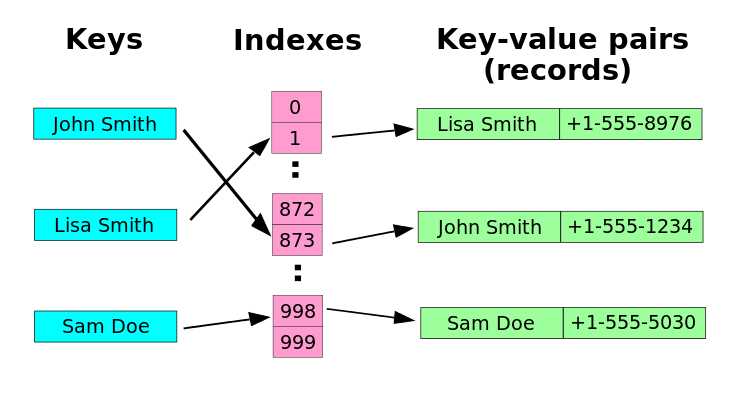
\includegraphics[scale=0.25]{img/hash_table}
\caption{Example of data insertion in a hash table}
\end{figure}
\end{frame}

\SlideSubSection{Collisions}
\begin{slide}{
\item The hash function might return duplicate values for two different keys, or for duplicate keys.
\item We add an element to the bucket for each collision.
\item \textbf{What happens if the bucket is full?} (\textit{overflow})
\pause
\item Add a list as overflow bucket. All overflowing entries are stored in the overflow bucket.
\item Extend the bucket array when needed.
}\end{slide}

\SlideSubSection{Performance (WHERE)}
\begin{slide}{
\item Consider the query on ships presented in the WHERE slides. Suppose we have a hash table on \texttt{firepower}.
\item \textbf{How many operations does the selection require?}
\pause
\item 1 to access the correct bucket, plus 3 operations to read the query in the same bucket = 4 operations vs 10 of non-indexed implementation.
}\end{slide}

\begin{frame}[fragile]{Performance (JOIN)}
\begin{itemize}
\item \textbf{How can the join be implemented?}
\pause
\end{itemize}
\begin{lstlisting}[language = Java]
for (p : projectiles)
  for (s : ships)
    if (s.name = p.target &&
        s.position = p.position)
         add <s.name,p.damage> to result
\end{lstlisting}
\begin{itemize}
\item We can index one of the tables and put the indexed query as inner query in the for-loop.
\end{itemize}
\end{frame}

\begin{slide}{
\item \textbf{What is the cost of the join with a hash index on} \texttt{name}\footnote{Assume that the index maps the starting letter of its position in the alphabet order and no collisions}?
\pause
\item For each record in \texttt{projectile} we need to access the bucket in the other table
\item The only record which matches in \texttt{ship} is \texttt{'Red 3'}.
\item We apply the hash function and read the entry in the hash table for 'Red 3'. This means $3 \cdot 2 = 6$ operations to select the ships in both table with the same name.
\item In total we have 6 + 30 operations = 36 operations (30 for the non-indexed attribute in the condition).
}\end{slide}

\begin{slide}{
\item \textbf{What if we also have an index on} \texttt{position}?
\pause
\item There is one entity in the \texttt{ships} table which matches the condition.
\item For each record in \texttt{projectiles} we look for a record in \texttt{ships} with the same position.
\item 2 records mismatch the position and one matches.
\item Accessing the mismatching records requires 2 operations (we only need to hash the search key to find it is not in the buckets). Accessing the matching record requires 2 operations. In total 4 operations.
\item With two indices we require only 6 + 4 = 10 operations.
}\end{slide}

\SlideSubSection{Drawbacks of hash tables}
\begin{slide}{
\item Useless if the condition is not an equality but an inequality (conditions on intervals).
\item Useless with ordering/grouping commands.
\item A lot of collisions require to extend the buckets/slow down the search if overflow buckets are used.
}\end{slide}

\SlideSection{Trees}
\SlideSubSection{Balanced trees}
\begin{slide}{
\item A graph is a set of vertices connected by edges.
\item A tree is a graph without cycles and connected (all nodes can be reached following connections from a starting node).
\item The top node is called \texttt{root}.
\item The nodes that are directly connected to a node and at a deeper level are called children. The children shares the same parent.
\item A node which does not have children is called \textit{leaf}.
\item A balanced tree is a tree where the leaves are all at the same level.
}\end{slide}

\SlideSubSection{2-3 Trees}
\begin{slide}{
\item Balanced tree.
\item Every node contains at most 2 entries
\item Every node has 2 or 3 children.
\item The keys in the left child are less than or equal to the keys in the parent.
\item The keys in the middle child are between the min and the max keys stored in the parent.
\item The keys in the right child are greater than or equal to the keys in the parent.
}\end{slide}

\begin{frame}{2-3 Trees}
\begin{figure}
\centering
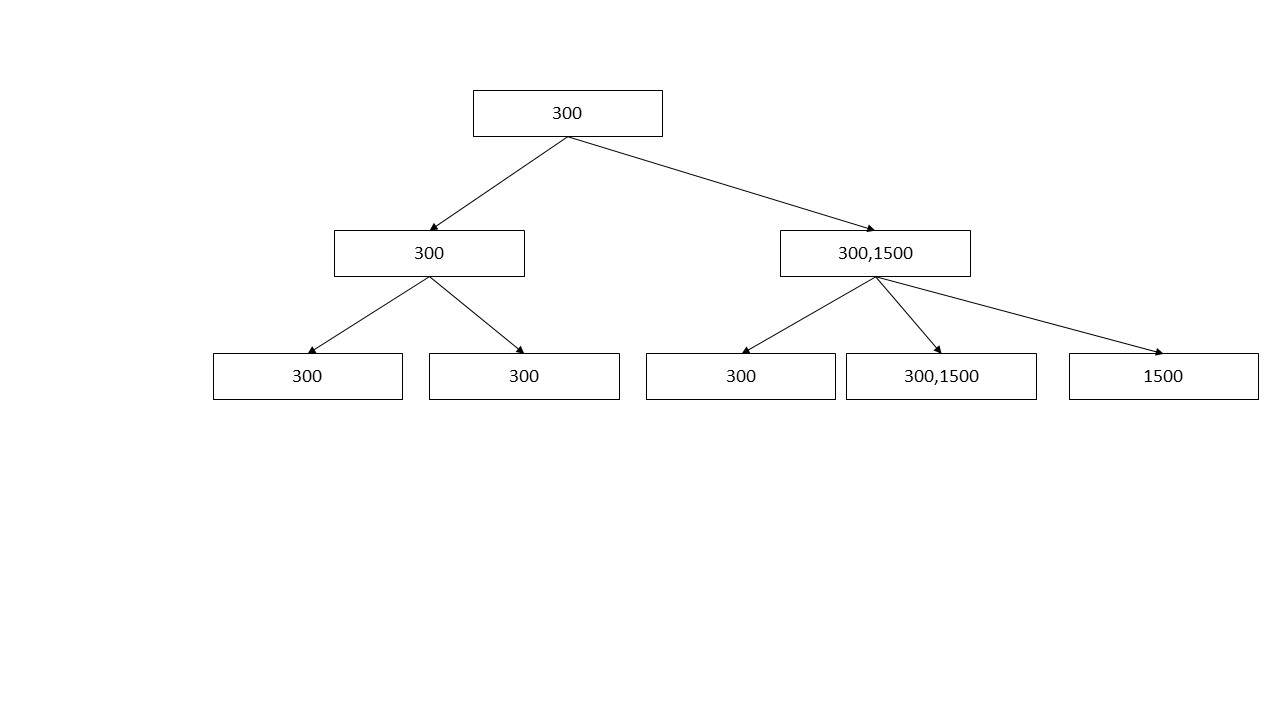
\includegraphics[scale=0.3]{img/tree2}
\caption{Index on \texttt{firepower}}
\end{figure}
\end{frame}

\SlideSubSection{Performance (WHERE)}
\begin{slide}{
\item Consider the query on ships presented in the WHERE slides. Suppose we have a 2-3 tree index on \texttt{firepower}.
\item \textbf{How many operations does the selection require?}
\pause
\item We follow the index and we find 3 entries, reading 4 nodes. We need 4 operations vs 10 operations without an index.
}\end{slide}

\SlideSubSection{Performance (JOIN)}
\begin{slide}{
\item \textbf{What is the cost of the join with a 2-3 tree index on} \texttt{name} in table \texttt{ships} (see the next slide for the index) \footnote{Assume that the index maps the starting letter of its position in the alphabet order}?
\pause
\item This time the inner table in the for-loop is \texttt{ships}.
\item We need to find 'Red 3' three times in the index. This requires to traverse the whole three 3 times and each time we access the record, for a total of 12 operations.
\item We have 12 operations vs the required 30 without indexing.
\item In total we have 42 operations vs 60 (\texttt{position} is not indexed).
\item This is a very unlucky case, since the entry is stored in a leaf. Imagine we were looking for "Red 4", we would need just 1 operation to get to the correct node.
}\end{slide}

\begin{frame}{Performance (JOIN)}
\begin{figure}
\centering
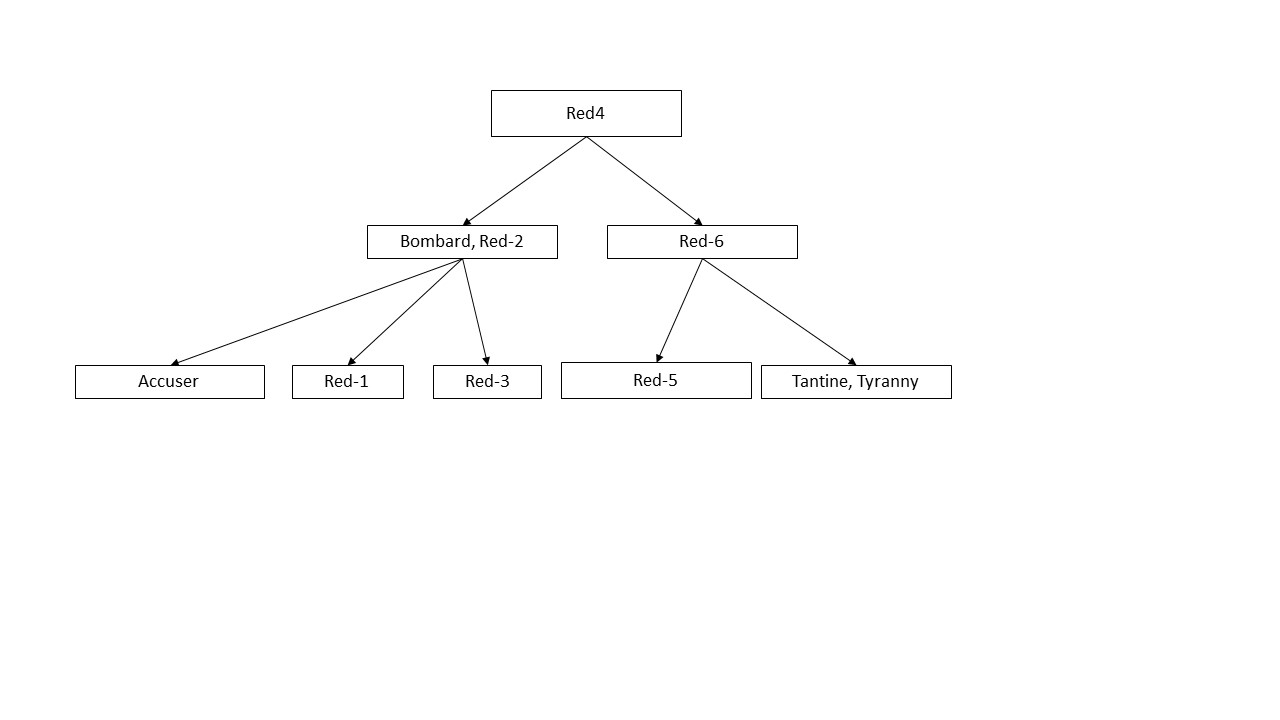
\includegraphics[scale=0.3]{img/tree1}
\caption{Index on \texttt{name}}
\end{figure}
\end{frame}

\begin{slide}{
\item \textbf{Can you guess what is the generalized formula for the number of operations to search for a key in a 2-3 tree?}
\pause
\item $\log_{2} N$ where $N$ is the number of entries.
}\end{slide}



\begin{frame}{Performance (JOIN)}
\begin{itemize}
\item \textbf{What if we also have an index on} \texttt{position} (see the next slide for the index)\footnote{Imagine that the key is generated by summing the components of the position}?
\pause
\item The position will not match for 2 out of 3 records in \texttt{projectile}. So we have to traverse 3 nodes in the tree twice for a total of 6 operations.
\item The last position will match and the entry is stored in the root so we need just 1 operation.
\item In total we have 7 operations.
\item With both indices we need 19 vs 60 operations without indices.
\end{itemize}
\end{frame}

\begin{frame}{Performance (JOIN)}
\begin{figure}
\centering
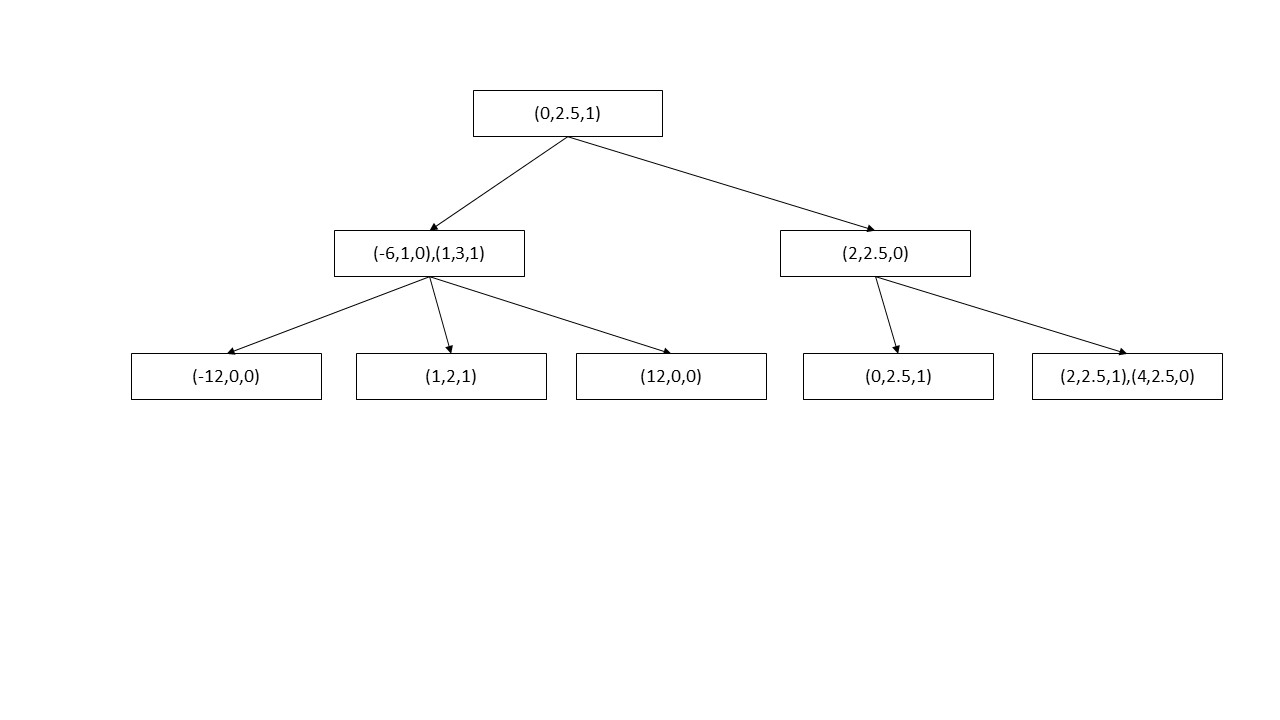
\includegraphics[scale=0.3]{img/tree3}
\caption{Index on \texttt{position}}
\end{figure}
\end{frame}

\SlideSubSection{Ordering/grouping with trees}
\begin{slide}{
\item A clustered index is an index where the record order in a file is the same in the index.
\item If the tree index is clustered we can use the tree for ordering/grouping.
\item Just traverse the tree. If the ordering is ascending then visit all the nodes starting from the leftmost and then moving to the rightmost.
\item This requires $N$ steps where $N$ is the number of entries in the index (vs $N \log N$ of a traditional ordering algorithm).
}\end{slide}

\begin{frame}{Ordering/grouping with trees}
\textbf{Exercise: order the \texttt{name} attributes in ascending order}.
\end{frame}

\begin{frame}{Ordering/grouping with trees}
\textbf{Exercise: order the \texttt{name} attributes in ascending order}.
\animategraphics[autoplay,loop,scale=0.35]{1}{img/order}{1}{10}
\end{frame}

\SlideSubSection{Overall evaluation of trees}
\begin{slide}{
\item Fast with conditions on intervals.
\item Fast with ordering/group by.
\item The worst case requires to scan $\log N$ entries before finding our entries (with Hash tables it is at most the size of the largest bucket).
}\end{slide}

\SlideSubSection{Golden rules of indexing}
\begin{slide}{
\item If most of the queries have selections/joins with equalities choose hash tables.
\item If most of the queries have selections/joins with inequalities choose trees.
\item If you can anticipate there will be a lot of mismatches in the comparisons choose hash tables.
\item If you anticipate there will be a lot of collisions (a lot of duplicate values) choose trees.
\item If you have a lot of queries with ordering/group by use clustered trees (otherwise do not use clustering).
}\end{slide}



\end{document}

\begin{slide}{
\item ...
}\end{slide}

\begin{frame}[fragile]
\begin{lstlisting}
...
\end{lstlisting}
\end{frame}
